 \part{Модуль 1.}

\section{
    Комплексные числа. Арифметические действия над комплексными числами. Возведение в степень и извлечение корня. Комплексная плоскость, модуль, аргумент. Формула Эйлера. Формула Муавра.
}

\subsection{
    Комплексные числа.
}

\begin{definition}
    \textbf{\textit{Комплексным числом $z$}} называется пара $(x, y)$ действительных чисел $x, y \in \RR$, для которой определены понятие равенства и операции сложения и умножения следующим образом:
    
    \begin{enumerate}[nosep]
        \item $z_1 = z_2 \iff x_1 = x_2$ и $y_1 = y_2$.
        \item $z_1 + z_2 = (x_1 + x_2, \thinspace y_1 + y_2)$.
        \item $z_1 \cdot z_2 = (x_1x_2 - y_1y_2, \thinspace \thinspace x_1y_2 + x_2y_1)$
    \end{enumerate}
\end{definition}

\begin{designation}
    $\CC$.
\end{designation}

\begin{definition}
    \textbf{\textit{Мнимой единицей}} называется число $i = (0, 1)$, причем ее квадратом, является пара $(-1, 0)$.
\end{definition}

\begin{definition}
    Комплексное число $\overline{z}$ называется \textbf{\textit{сопряженным}} к $z$, если $\overline{z} = x - iy$, $z = x + iy$.
\end{definition}

\textbf{Свойства комплексного сопряжения.}

\begin{enumerate}[label={\arabic*°.}]
    \item $\overline{z + w} = \overline{z} + \overline{w}.$
    
    $\overline{z + w} = \overline{(a_1 + b_1 i) + (a_2 + b_2 i)} = \overline{(a_1 + a_2) + (b_1 + b_2) i} = (a_1 + a_2) - (b_1 + b_2)i = (a_1 - b_1 i) + (a_2 - b_2 i) = \overline{z} + \overline{w}.$
    
    \item $\overline{zw} = \overline{z} \cdot \overline{w}.$
    
    $\overline{z} \cdot \overline{w} = (a_1 - b_1 i) (a_2 - b_2 i) = (a_1 a_2 - b_1 b_2) - (a_1 b_2 + a_2 b_1) i = \overline{zw}.$

    \item $\overline{\overline{z}} = z.$

    $\overline{\overline{z}} = \overline{\overline{a + bi}} = \overline{a - bi} = a + bi = z.$
\end{enumerate}


\newpage


\subsection{
    Арифметические действия над комплексными числами.
}

\begin{itemize}[nosep]
    \item $z_1 + z_2 = x_1 + x_2 + i(y_1 + y_2)$.
    \item $z_1 - z_2 = x_1 - x_2 + i(y_1 - y_2)$.
    \item $z_1 \cdot z_2 = (x_1 + iy_1)(x_2 + iy_2) = x_1x_2 + ix_1y_2 + ix_2y_1 - y_1y_2 = x_1x_2 - y_1y_2 + i(x_1y_2 + x_2y_1)$.
    \item $\frac{z_1}{z_2} = \frac{x_1 + iy_1}{x_2 + iy_2} = \frac{(x_1 + iy_1)(x_2 - iy_2)}{x_2^2 + y_2^2} = \underbrace{\frac{x_1x_2 + y_1y_2}{x_2^2 + y_2^2}}_{\text{Re}(\frac{z_1}{z_2})} + i\underbrace{\frac{x_2y_1 - x_1y_2}{x_2^2 + y_2^2}}_{\text{Im}(\frac{z_1}{z_2})}$.
\end{itemize}

\subsection{
    Возведение в степень и извлечение корня.
}

$z^n = w$

$w = |w|e^{i\varphi}$

$z = \sqrt[n]{|w|} \cdot e^{i \frac{\varphi + 2 \pi k}{n}}, \quad k = 0, 1, \ldots, n - 1.$

При нахождении корня $n$ степени из комплексного числа получается ровно $n$ чисел, лежащих на окружности радиусом $\sqrt[n]{|w|}$ и образующих правильный $n$-угольник.

\subsection{
    Формула Эйлера.
}

$z = |z|(\cos \varphi + i \sin \varphi)$ — тригонометрическая форма записи.

$e^{i\varphi} = \cos \varphi + i \sin \varphi$ — \textbf{формула Эйлера}.

$z = |z|e^{i\varphi}$ — показательная форма записи.


\subsection{
    Формула Муавра.
}

$z^n = |z|^n e^{in\varphi} = r^n(\cos n \varphi + i \sin n \varphi)$ — \textbf{формула Муавра}.


\newpage


\subsection{
    Комплексная плоскость, модуль, аргумент.
}

\begin{definition}
    \textbf{\textit{Комплексной плоскостью}} называется плоскость, образованная комплексными числами, у которой ось $Ox$ образована действительными числами, а ось $Oy$ - мнимыми числами.
\end{definition}

\begin{figure}[H]
    \centering
    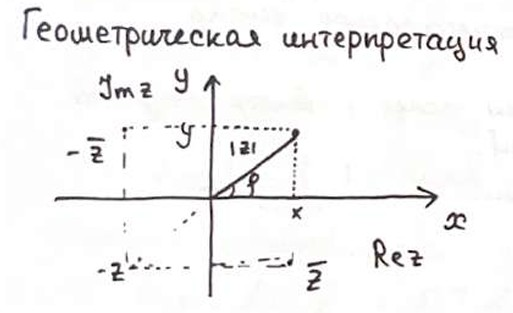
\includegraphics[scale=0.55]{images/1_1.jpg}
    \label{fig:picture_1_1}
\end{figure}


\begin{definition}
    \textbf{\textit{Модулем числа $z = x + iy$}} называется вещественное число $|z| = \sqrt{x^2 + y^2}$ (то есть длина соответствующего вектора).
\end{definition}

\textbf{Свойства.}

\begin{enumerate}[label={\arabic*°.}]
    \item $|z| \geq 0$, причем $|z| = 0 \iff z = 0$.
    \item $|z + w| \leq |z| + |w|$ (неравенство треугольника).

    Пусть $z = a + bi$, $w = c + di$.
    \begin{align*}
        |z + w| &\leq |z| + |w| \\
        \sqrt{(a + c)^2 + (b + d)^2} &\leq \sqrt{a^2 + b^2} + \sqrt{c^2 + d^2} \\
        (a + c)^2 + (b + d)^2 &\leq a^2 + b^2 + c^2 + d^2 + 2\sqrt{(a^2 + b^2)(c^2 + d^2)} \\
        ac + bd &\leq\sqrt{(a^2 + b^2)(c^2 + d^2)} \\
        ac + bd &\leq\sqrt{(ac)^2 + (ad)^2 + (bc)^2 + (bd)^2} \\
        (ac)^2 + (bd)^2 + 2acbd &\leq (ac)^2 + (ad)^2 + (bc)^2 + (bd)^2 \\
        2acbd &\leq (ad)^2 + (bc)^2 \\
        0 &\leq (ad)^2 + (bc)^2 - 2abcd \\
        0 &\leq (ad - bc)^2
    \end{align*}
    \item $z \overline{z} = |z|^2$.

    $z \overline{z} = (a + bi)(a - bi) = a^2 - (bi)^2 = a^2 + b^2 = |z|^2$
    \item $|zw| = |z||w|$.

    $|zw|^2 = (zw) \cdot (\overline{zw}) = z \cdot w \cdot \overline{z} \cdot \overline{w} = |z|^2 |w|^2$.
\end{enumerate}


\subsubsection*{
    Аргумент комплексного числа.
}


Пусть $z = a + bi \in \CC$, $z \neq 0$.

Тогда, $z = |z| \left(\frac{a}{|z|} + \frac{b}{|z|}i\right)$, при этом $\left(\frac{a}{|z|}\right)^2 + \left(\frac{b}{|z|}\right)^2 = (\frac{a}{\sqrt{a^2 + b^2}})^2 + (\frac{b}{\sqrt{a^2 + b^2}})^2 = \frac{a^2}{a^2 + b^2} + \frac{b^2}{a^2 + b^2} = \frac{a^2 + b^2}{a^2 + b^2} = 1.$

Значит, $\frac{a}{|z|}$ и $\frac{b}{|z|}$ являются синусом и косинусом некоторого угла.

\begin{definition}
    \textbf{\textit{Аргументом числа}} $z = a + bi \in \CC \setminus \{0\}$ называется любое число $\phi \in \RR$, такое что
    \begin{equation*}
        \cos \phi = \frac{a}{|z|} = \frac{a} {\sqrt{a^2 + b^2}}.
    \end{equation*}

    \begin{equation*}
        \sin \phi = \frac{b}{|z|} = \frac{b}{\sqrt{a^2 + b^2}}.
    \end{equation*}

    В геометрических терминах, $\phi$ есть угол между положительным направлением оси $Ox$ и вектором с началом в точке $0$ и концом в точке $z$.
\end{definition}

\begin{comment}
    Таких чисел бесконесно много, причем такие числа отличаются на $2\pi k, k \in \ZZ$.
\end{comment}
